\documentclass[12pt]{article}
\usepackage[a4paper, margin=1in]{geometry}
\usepackage{hyperref}
\usepackage{graphicx}
\usepackage[serbian]{babel}
\usepackage[T2A]{fontenc}
\usepackage[utf8]{inputenc}

\sloppy

\begin{document}

\bibliographystyle{plain} 


\begin{center}
    \large\textbf{Математички факултет} \\
    \large\textbf{Универзитет у Београду}
    
    \vspace{3cm}
    
    \Large\textbf{Семинарски рад} \\
    \large У оквиру курса Истраживање података 2
    
    \vspace{3cm}
    
    \LARGE\textbf{Тема:} \\
    \Large Истраживање образаца у патогеним острвима секвенци \textit{Escherichia coli} и \textit{Helicobacter pylori}
    
    \vspace{4cm}
    
    \begin{minipage}{0.4\textwidth}
        \begin{flushleft}
            \large\textbf{Професор:} \\
            \large Ненад Митић
        \end{flushleft}
    \end{minipage}
    \begin{minipage}{0.4\textwidth}
        \begin{flushright}
            \large\textbf{Студенти:} \\
            \large Вељко Продан, 163/2019 \\
            \large Маја Миленковић, 160/2019
        \end{flushright}
    \end{minipage}

    \vfill
    
    \large\textbf{Мај 2024}
    
\end{center}

\newpage

\tableofcontents

\addto\captionsserbian{
    \renewcommand\contentsname{Садржај}
}

\newpage

\section{Увод}

\subsection{Патогена острва}

Патогена острва (\textit{Pathogenicity island} - PAI) су посебни генетски елементи присутни на хромозомима великог броја бактеријских патогена. PAI кодирају различите факторе вируленције и обично су одсутни код непатогених сојева исте или блиско сродних врста. Сматрају се подкласом геномских острва која се стичу хоризонталним преносом гена путем трансдукције, коњугације и трансформације, и пружају "квантне скокове" у микробној еволуцији, што доприноси способности микроорганизама да еволуирају \cite{Gal-Mor2006-dv}. 

Једна бактеријска врста може имати више од једног PAI. PAI су кластери гена уграђени у геном патогених организама, хромозомално или екстрахромозомално. Као тип мобилног генетичког елемента, PAI могу варирати од 10-200 кб. Они носе гене који им омогућавају да производе различите факторе вируленције, укључујући адхезине, токсине, системе секреције и друге елементе који им помажу да се вежу за ћелије домаћина, избегну имуни систем и изазову болест \cite{Schmidt2004-xj}. Подаци засновани на бројним секвенцираним бактеријским геномима показују да су PAI присутни у широком спектру грам-позитивних и грам-негативних бактеријских патогена људи, животиња и биљака. Недавна истраживања усмерена на PAI довела су до идентификације многих нових фактора вируленције које ове врсте користе током инфекције својих домаћина \cite{Gal-Mor2006-dv}.

\subsection{Ешерихија коли}

Ешерихија коли (Escherichia coli) је разноврсна бактеријска врста која обухвата како безопасне коменсалне сојеве, тако и патогене сојеве који се налазе у гастроинтестиналном тракту људи и топлокрвних животиња. Патогеност Ешерихије коли, која се постиже хоризонталним трансфером гена који одређују факторе вируленције, омогућава овој бактерији да постане врло разноврстан и адаптибилан патоген одговоран за цревне или ванцревне болести код људи и животиња. Сходно томе, сојеви Е. коли могу се класификовати у три групе: коменсалне/пробиотске сојеве, интестинално патогене сојеве и екстраинтестинално патогене сојеве.

Растућа количина информација о ДНК секвенцама, генерисаних у "ери геномике", помогла је у повећању разумевања фактора и механизама укључених у диверзификацију ове бактеријске врсте \cite{Desvaux2020-mx}. 

\subsection{Хеликобактер пилори}

Хеликобактер пилори је грам-негативни патоген спиралног облика који колонизује антрум и корпус желуца. У последњој деценији, идентификовани су бројни фактори вируленције. Ови елементи омогућавају бактерији да преживи у изузетно киселој средини гастроинтестиналног тракта, доспе до неутралније средине слузног слоја и одупре се имунолошком одговору човека, што резултира перзистенцијом \cite{2022helicobacter}.

Сојеви Хеликобактер пилори показују висок степен генетске хетерогености због геномских преуређења, тачкастих мутација, убацивања и/или брисања гена. Генетички јединствене варијанте једног соја присутне су у желуцима сваког човека, а генетски састав ових популација може се мењати током времена. Ова адаптабилност доприноси и њеној високој заразности \cite{Noto2012-rr}.

Већина инфекција се јавља у детињству, а само мали проценат инфекција напредује до тежих стања. Инфекција овом бактеријом може изазвати различите гастроинтестиналне проблеме, укључујући хронични гастритис, чир на дванаестопалачном цреву, па чак и рак. Хеликобактер пилори је веома заразна бактерија \cite{2022helicobacter}.

\section{Алгоритми истраживања образаца}

\subsection{TF-IDF}

TF-IDF\cite{Liu2018-oa} (Term Frequency Inverse Document Frequency) алгоритам
 је
статистички метод који се користи за процену важности речи
за документ или категорију у скупу датотека или корпусу. 

Главна идеја је да ако се нека реч или фраза често појављује у
чланку, а ретко се налази у другим члaнцима, сматра се
да реч или фраза има добру способност разликовања класе
и погодна је за класификацију. То је најчешће коришћена
функција за израчунавање тежине речи у тренутном
векторском моделу простора. Углавном се састоји од
два дела, а то су учесталост речи и инверзна учесталост
текста. Учесталост речи се односи на број појављивања
дате речи у датотеци. Инверзна учесталост датотеке представља
меру опште важности речи. Инверзна учесталост речи се рачуна деобом
укупног броја докумената са бројем
докумената који садрже тај термин, а затим се логаритмује
резултат количника. Формуле за учесталост речи (TF) и
инверзну учесталост текста (IDF) су следеће:
$$\mathrm{tf}_{i,j} = \frac{n_{i,j}}{\sum_{k} n_{k,j}}$$

$n_{i,j}$  је број појављивања речи ti у датотеци $d_{j}$,
$\sum_{k} n_{k,j}$ је збир појављивања свих речи у датотеци
$d_{j}$.

$$\mathrm{idf}_i = \log \left(\frac{|D|}{|\{j : t_i \in d_j\}|}\right) $$

$|D|$ је укупан број датотека у корпусу, $|\{j : t_i \in d_j\}|$
је број докумената који садрже реч $t_{i}$. Ако
речи нема у корпусу, то ће довести до деобе са нулом. Зато се
уопштено користи 1+$|\{j : t_i \in d_j\}|$.

$$\mathrm{tfidf}_{i,j} = \frac{\mathrm{tf}_{i,j} \times \mathrm{idf}_{i}}{\sqrt{\sum_{t_i \in d_j} \left[\mathrm{tf}_{i,j} \times \mathrm{idf}_i\right]^2}}$$


$\mathrm{tfidf}_{i,j}$ је тежина речи ${t}_{i}$. Може се видети да висока
учесталост речи у одређеној датотеци и ниска учесталост датотеке
речи у целом скупу датотека могу генерисати високу TF-IDF вредност. 

\subsection{NOSEP}

NOSEP\cite{8053457} (Nonoverlapping Sequence Pattern Mining With Gap Constraints) представља исцрпан алгоритам за рударење образаца секвенци који користи Nettree структуру података. Ова структура омогућава прецизно израчунавање учесталости појављивања одређеног обрасца унутар дате секвенце, узимајући у обзир услов непреклапања. Приликом рударења образаца секвенци, два главна фактора која утичу на перформансе су израчунавање подршке и смањење простора кандидата образаца. 

За израчунавање подршке, користи се NETGAP алгоритам. NETGAP треба да  разликује знакове у секвенци који се могу поново користити за упаривање образаца, да би се испунио услов непреклапања. Овај изазов се односи на немогућност једноставне замене одговарајућих знакова у секвенци знаком "X", јер би то спречило проналажење будућих непреклапајућих појава. Стога, NETGAP мора ефикасно разликовати знакове који се могу поново користити.

Да би се превазишао наведени проблем и имплементирао алгоритам без претраге уназад, предлаже се коришћење Nettree структуре података. Nettree се конструише на основу обрасца и секвенце, а затим се итеративно проналазе минималне путање које представљају појаве обрасца. После сваке итерације, минимална путања и неважећи чворови се уклањају из дрвета. Овај процес се понавља док дрво не постане празно, гарантујући потпуно проналажење свих појава обрасца.

\begin{center}
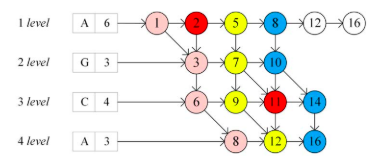
\includegraphics[width=0.6\linewidth]{images/nettree.png}
\end{center}

Са друге стране, NOSEP алгоритам користи приступ раста образаца за смањење простора кандидата образаца, који се показао ефикаснијим од приступа претраге у ширину и дубину. NOSEP поседује Apriori својство, што имплицира да ако подобразац није фреквентан, његов надобразац такође не може бити фреквентан. Захваљујући овом својству, простор кандидата образаца се ефикасно редукује.

NOSEP започиње рад проналажењем свих честих узорака дужине 1, а затим итеративно генерише кандидатске узорке растуће дужине комбиновањем честих узорака краћих дужина. За сваки кандидатски узорак, његова подршка се израчунава коришћењем NETGAP алгоритма и Nettree структуре података. Кандидати чија подршка задовољава минимални праг се додају у скуп честих узорака за ту дужину. Овај процес се наставља док се не може пронаћи више честих узорака. На крају, NOSEP враћа унију свих пронађених честих узорака свих дужина, ефикасно рударећи комплетан скуп честих секвенцијалних образаца.

\section{Примена алгоритама}

\textbf{\large TF-IDF}

Блабла

\textbf{\large NOSEP}


Улаз NOSEP алгоритма је кодирана секвенца карактера и пет параметара:

1. минимално ограничење дужине \textit{minlen}

2. максимално ограничење дужине \textit{maxlen}

3. минимално ограничење празнине \textit{mingap}

4. максимално ограничење празнине \textit{maxgap}

5. задати праг минималне подршке \textit{minsup}\\


У оквиру пројекта, вредности наведених параметара су биле постављене на следећи начин: минимална дужина 4, максимална дужина 100, минимална празнина 0, максимална празнина 0 и праг минималне подршке 2.

NOSEP је потом покренут над свим геномима и њиховим острвима ради проналажења образаца у оквиру острва који се не налазе ван острва. Међутим, да би се осигурало да пронађени обрасци буду јединствени за острва, уклоњени су они обрасци који су били присутни и ван острва, у свим осталим геномима.


\newpage
\bibliography{seminarski}

\end{document}

